\documentclass{bioinfo}
\copyrightyear{2005}
\pubyear{2014}

\graphicspath{{./figures/}}

\usepackage{color}
\usepackage{multirow}

\begin{document}
\firstpage{1}

\title[Global Optimization-based Inference of Chemogenomic Features]{Global Optimization-based Inference of Chemogenomic Features from Drug-Target Interactions}
\author[Zu,S. \textit{et~al}]{Songpeng Zu\,$^{1}$, Ting Chen\,$^{1,2}$, Shao Li\,$^{1}$\footnote{to whom correspondence should be addressed}}
\address{$^{1}$MOE Key Laboratory of Bioinformatics and Bioinformatics Division, TNLIST/Department of Automation, Tsinghua University, Beijing 100084, China.\\
$^{2}$Molecular and Computational Biology Program, Department of Biological Sciences, University of Southern California, Los Angeles, California 90089, USA.}

\history{Received on XXXXX; revised on XXXXX; accepted on XXXXX}

\editor{Associate Editor: XXXXXXX}

\maketitle

\begin{abstract}
\section{Motivation:}
Gaining insight into chemogenomic drug-target interactions, such as those involving the substructures of synthetic drugs and protein domains, is important in fragment-based drug discovery and drug repositioning. Previous studies evaluated the interactions locally, thereby ignoring the competitive effects of different substructures or domains, but this could lead to high false-positive estimation, calling for a computational method that presents more predictive power.
\section{Results:}
A statistical model, termed Global optimization-based InFerence of chemogenomic features from drug-Target interactions, or GIFT, is  proposed herein to evaluate substructure-domain interactions globally {\color{red}such that all substructure-domain contributions to drug-target interaction are analyzed simultaneously.} Combinations of different chemical substructures were included since they may function as one unit. When compared to previous methods, GIFT showed better interpretive performance, and performance for the recovery of drug-target interactions was good. {\color{red}Among 53 known drug-domain interactions, 81\% were accurately predicted by GIFT.} Eighteen of the top 100 predicted combined substructure-domain interactions had corresponding drug-target structures in the Protein Data Bank database, and 15 out of {\color{red}the 18} had been proved. GIFT was then implemented to predict substructure-domain interactions based on drug repositioning. For example, the anticancer activities of tazarotene, adapalene, acitretin and raloxifene were identified. In summary, GIFT is a global chemogenomic inference approach and offers fresh insight into drug-target interactions.
\section{Availability:}
The source codes can be found at\\ \href{http://bioinfo.au.tsinghua.edu.cn/software/GIFT/}{http://bioinfo.au.tsinghua.edu.cn/software/GIFT}.
\section{Contact:} \href{shaoli@mail.tsinghua.edu.cn}{shaoli@mail.tsinghua.edu.cn}
\end{abstract}

\section{Introduction}
\begin{figure*}
\centerline{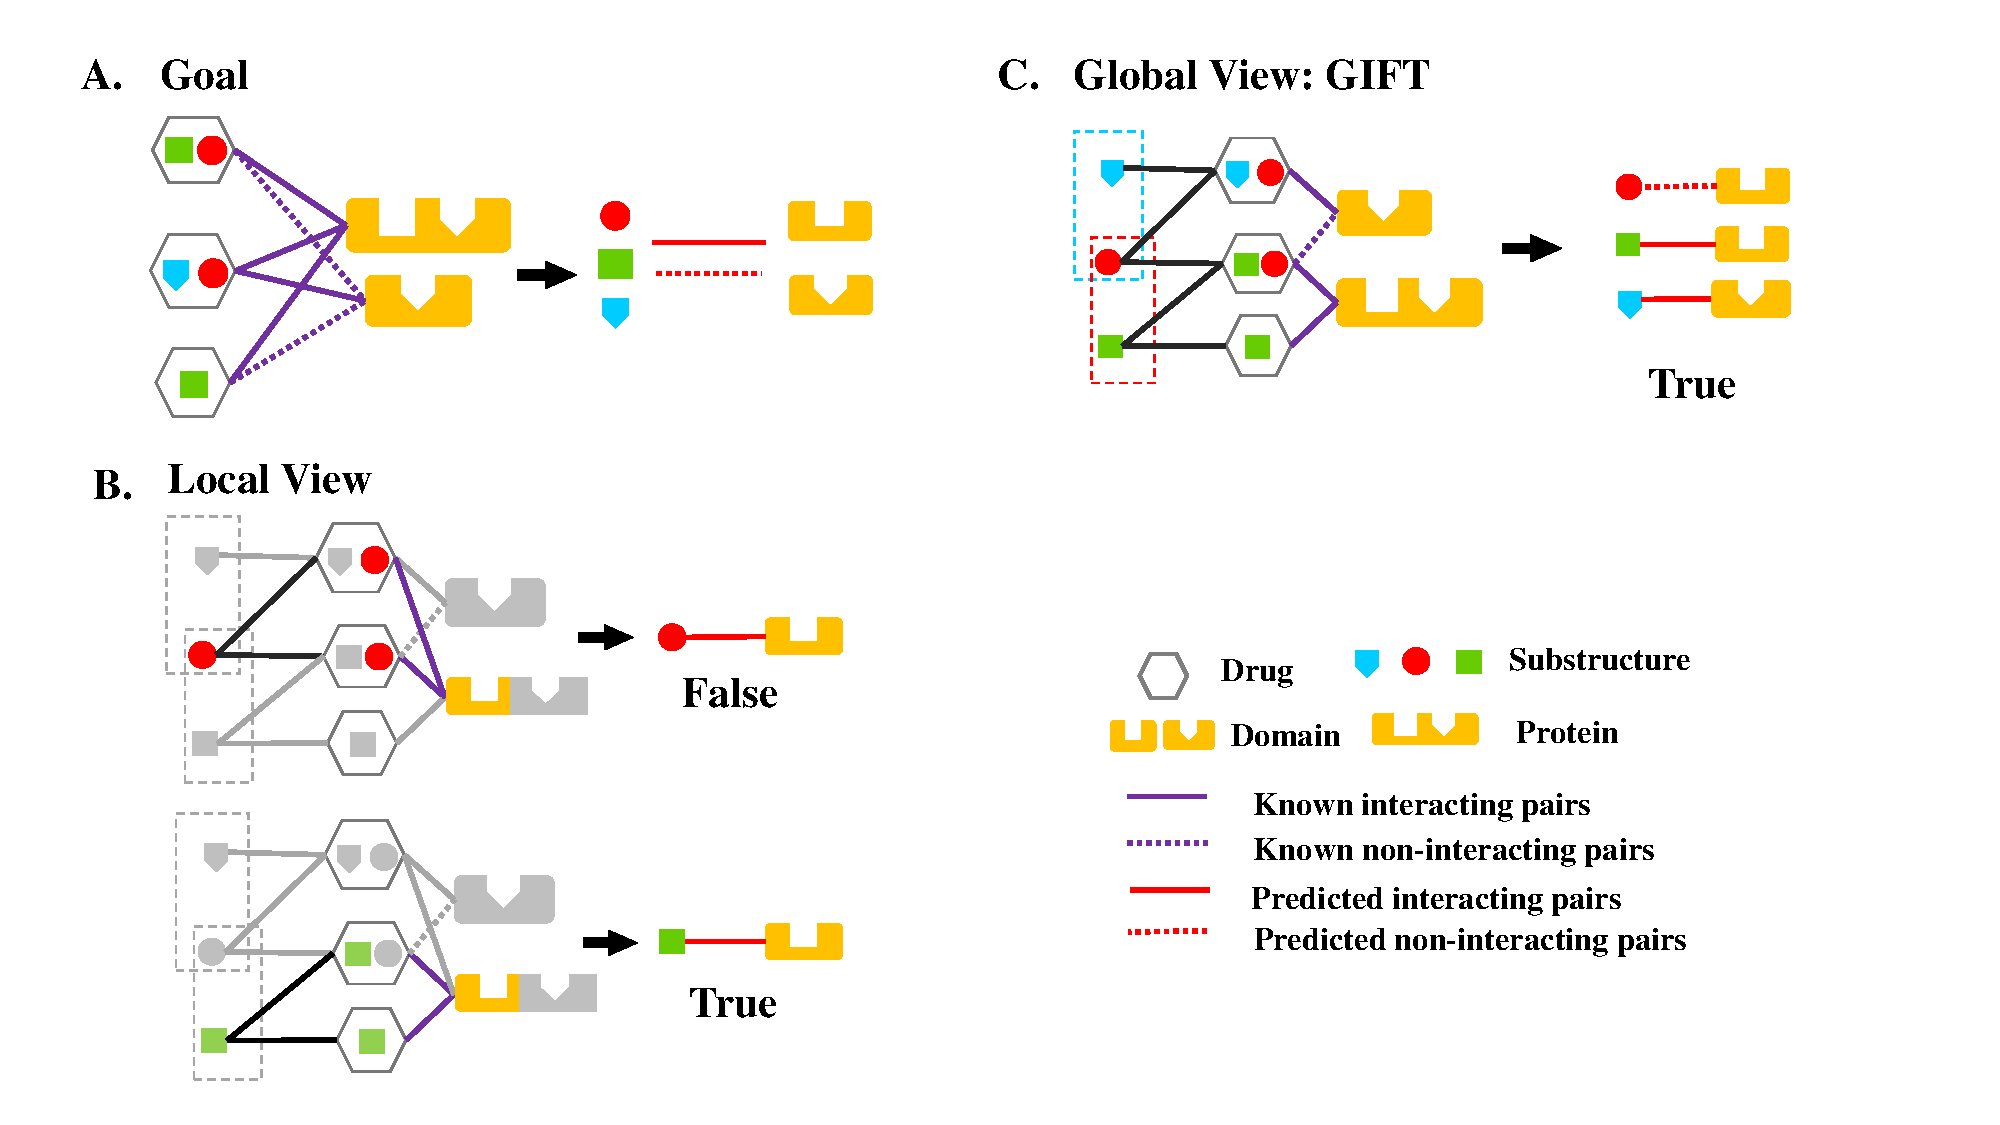
\includegraphics[width=\textwidth]{explains_v2}}
\caption{{\color{red}Schematic diagram of GIFT. A. The goal of GIFT is to infer the underlying drug substructure-protein domain interactions, given a set of drug-protein interactions. B. The local view of previous approaches that test one pair of substructure-domain at a time while ignoring other substructures or protein domains. C. The global view of GIFT that considers contributions of all substructure-domain pairs to the given set of drug-target interactions.}
\label{fig:01}}
\end{figure*}

Protein domains are independent folding structures and form different proteins as the functional units (\citealp{Chothia84}). Compared with sequence similarity, domain structures are much more conserved among proteins (\citealp{Koehn2005}). Compound chemical substructures, or functional scaffolds, are the basic structural and functional building blocks of small molecules (\citealp{Bemis96}). According to Bredel and Jacoby (2004), chemogenomics, or chemical genomics, involves the systematic screening of targeted chemical libraries of small molecules against individual drug target families with the goal of identifying new drugs and drug targets. Thus, gathering chemogenomic data about protein domains and the chemical substructures of drugs underlying drug-target interactions could foster the development of fragment-based drug discovery, drug repositioning and the understanding of drug-induced side effects (\citealp{Murray09}; \citealp{Yamanishi2011}; \citealp{duran13}), thereby supplementing the network pharmacology methods of target prediction (\citealp{ZhaoS2010}).

Among 1584 FDA-approved drugs and 89 nutraceuticals from the DrugBank database (\citealp{DrugBank2008}), only 30\% of them are contained in the Protein Data Bank (PDB) database (\citealp{Berman00}; \citealp{Gallina2013}). The large gap between the number of known binding positions and the total number of drug-target pairs calls for computational models to bridge them. Such computational models can be classified as structure-based methods and nonstructure-based methods. Structure-based methods, such as docking, have been developed over the course of many years, but they are constrained by the dependence on three dimensional structures of proteins (\citealp{Sousa2013}; \citealp{Yang2013}). In recent years, several nonstructure-based methods, which are not limited by the structure information��have been developed, along the accumulation of large-scale database in both chemistry and biology.

Yamanishi and colleagues (2011) developed a sparse canonical correspondence analysis method to extract the associated sets of chemical substructures and protein domains from drug-target interactions, but the amount of detectable protein domains was relatively small. Takigawa and colleagues (2011) applied graph mining and sequence mining to automate the search for significant substructure patterns, leading to the interpretation of polypharmacology in drug-target network. The substructures in drugs or proteins did not need to be defined from the literatures. {\color{red}However, protein substructures, which are generally composed of two or three residues, were difficult to correlate with biological interpretations.} Tabei and colleagues (2012) treated this question as a classification problem in machine learning. They used the logistic regression and support vector machine (SVM) algorithm to seek the drug chemical substructures and protein domains pairs that could be used to determine whether drugs and proteins interact or not. This method showed good results in predicting drug-target interactions.

However, none the methods noted above was able to evaluate uncertainty or variance of results, and they also ignored the possible combinations of drug chemical substructures that bind to protein domains as a whole. More importantly, the competitive effects of different substructure-domain interactions have never been considered since prediction has, thus far, been performed locally.

Therefore, in this article, a Global optimization-based InFerence of chemogenomic features from drug-Target interactions, termed GIFT, was proposed (Figure \ref{fig:01}). {\color{red}Since different drug chemical substructures and protein domains may competitively contribute to drug-target interactions, GIFT takes into consideration all the substructure-domain interactions} and treats them as latent variables leading to drug-target interactions.{\color{red} A substructure-domain interaction is defined as a direct physical interaction between a chemical substructure and a protein domain, for example, a hydrogen bond between an atom in a chemical substructure and an atom in an amino acids (\citealp{Gallina2013}).} It should be noted that because some drug-target interactions have not been recorded in DrugBank, {\color{red} we incorporated two parameters, namely {\it fp}  (false positive rate) and {\it fn}  (false negative rate), to describe data inaccuracy and incompleteness.} Then the substructure-domain contributions to different drug-target pairs were globally analyzed by {\color{red}the Expectation-Maximum (EM) algorithm framework, a statistical method to find the maximum likelihood estimates when the latent variables exist (\citealp{dempster1977maximum}).} Variances in results were calculated by the observed Fisher Information (\citealp{efron78}). In the following report, GIFT was extended to solving the problems with combinations of different drug chemical substructures based on the likelihood that some may function together. More than 700 substructure-domain interactions were found by GIFT. Some were validated by the PDB database. Our approach is a promising method for investigating drug-target binding positions and contributes to our understanding in this field.

\section{Results}
\subsection{Robust Analysis of \textit{fn} and \textit{fp} on Recovering Drug-Target Interactions}
\begin{table}
\processtable{Performance on recovery of drug-target interactions. \label{Tab:01}}
{\begin{tabular}{ccccc}\toprule
\textbf{Ratio} & \textbf{GIFT} & \textbf{L1-Log} & \textbf{L1-SVM} & \textbf{SCCA}\\\midrule
1 & 0.835 (0.006) & 0.829 (0.001) & 0.830 (0.001) & 0.798 (0.002)\\
5 & 0.847 (0.006) & 0.838 (0.001) & 0.855 (0.001) & 0.798 (0.002)\\\botrule
\end{tabular}
}{{\color{red}The values are the mean areas under the ROC curves with the standard variances}. Ratio is the proportion of negative samples over the total number of training samples.}
\end{table}

\begin{table}
\processtable{Performance on recovery of drug-target interactions on different combinations of the two fixed parameters. \label{Tab:02}}
{\begin{tabular}{ccccccc}\toprule
\emph{\textbf {fn}} &0.10 & 0.10& 0.40& 0.40&0.80& 0.80\\
\emph{\textbf{fp}}&0.0001& 0.001 &0.0001& 0.001& 0.0001 &0.001\\\midrule
 &0.845  & 0.837  & 0.846  & 0.838  & 0.847  & 0.840 \\
 &(0.006) & (0.005) & (0.006)& (0.005)&(0.006) &(0.005) \\ \botrule
\end{tabular}}{The values are the mean areas under the ROC curves with the standard variances.}
\end{table}

As noted above, two parameters, \textit{fp} (false positive rate) and \textit{fp}   (false negative rate) should be given in GIFT. Based on the assumptions in GIFT (See Methods), we roughly estimated that the value of fn was no less than 0.4 and the value of \textit{fp} was no more than 0.001 (See Methods).

In order to analyze the robustness of GIFT with different parameters, we used 5-fold cross validation to detect the recoveries of drug-target interactions on different combinations of \textit{fn} and \textit{fp}. Here the negative samples were randomly selected from the drug-protein pairs without interacting records. The results showed that the performance for recovering drug-target interactions remained stable for different combinations of \textit{fn} and \textit{fp} ({\color{red}See Table \ref{Tab:02}}). In GIFT, \textit{fn} was set as 0.85 and \textit{fp} was set as 0.0001.

Following the same cross validation procedure above, we compared GIFT with previous methods, namely, L1-log, L1-SVM (\citealp{Tabei2012}), SCCA (\citealp{Yamanishi2011}) and the association method (See Methods), based on their performance for recovery of drug-target interactions. The association method was a naive approach to inference of  substructure-domain interactions. The area under the ROC curve (AUC) of the association method is 0.72 (data not shown). {\color{red}Based on the AUC (See Table \ref{Tab:01}), GIFT performed better than the association method, L1-Log method, as well as SCCA, and it was comparable to L1-SVM for predicting drug-protein interactions.}

Although a large number of substructure-domain interactions were extracted by the previous methods, for example, more than 350,000 interactions by SCCA (\citealp{Yamanishi2011}), and around 5,000 interactions by L1-SVM (\citealp{Tabei2012}), it was difficult to assess the accuracy of these interactions. In the following sections, we demonstrate that GIFT not only perform better for drug-target predictions, but also provided better interpretation of the extracted substructure-domain interactions.

\subsection{Performance of Prediction on Drug-Domain Interactions}
\begin{figure*}[htb]
\centerline{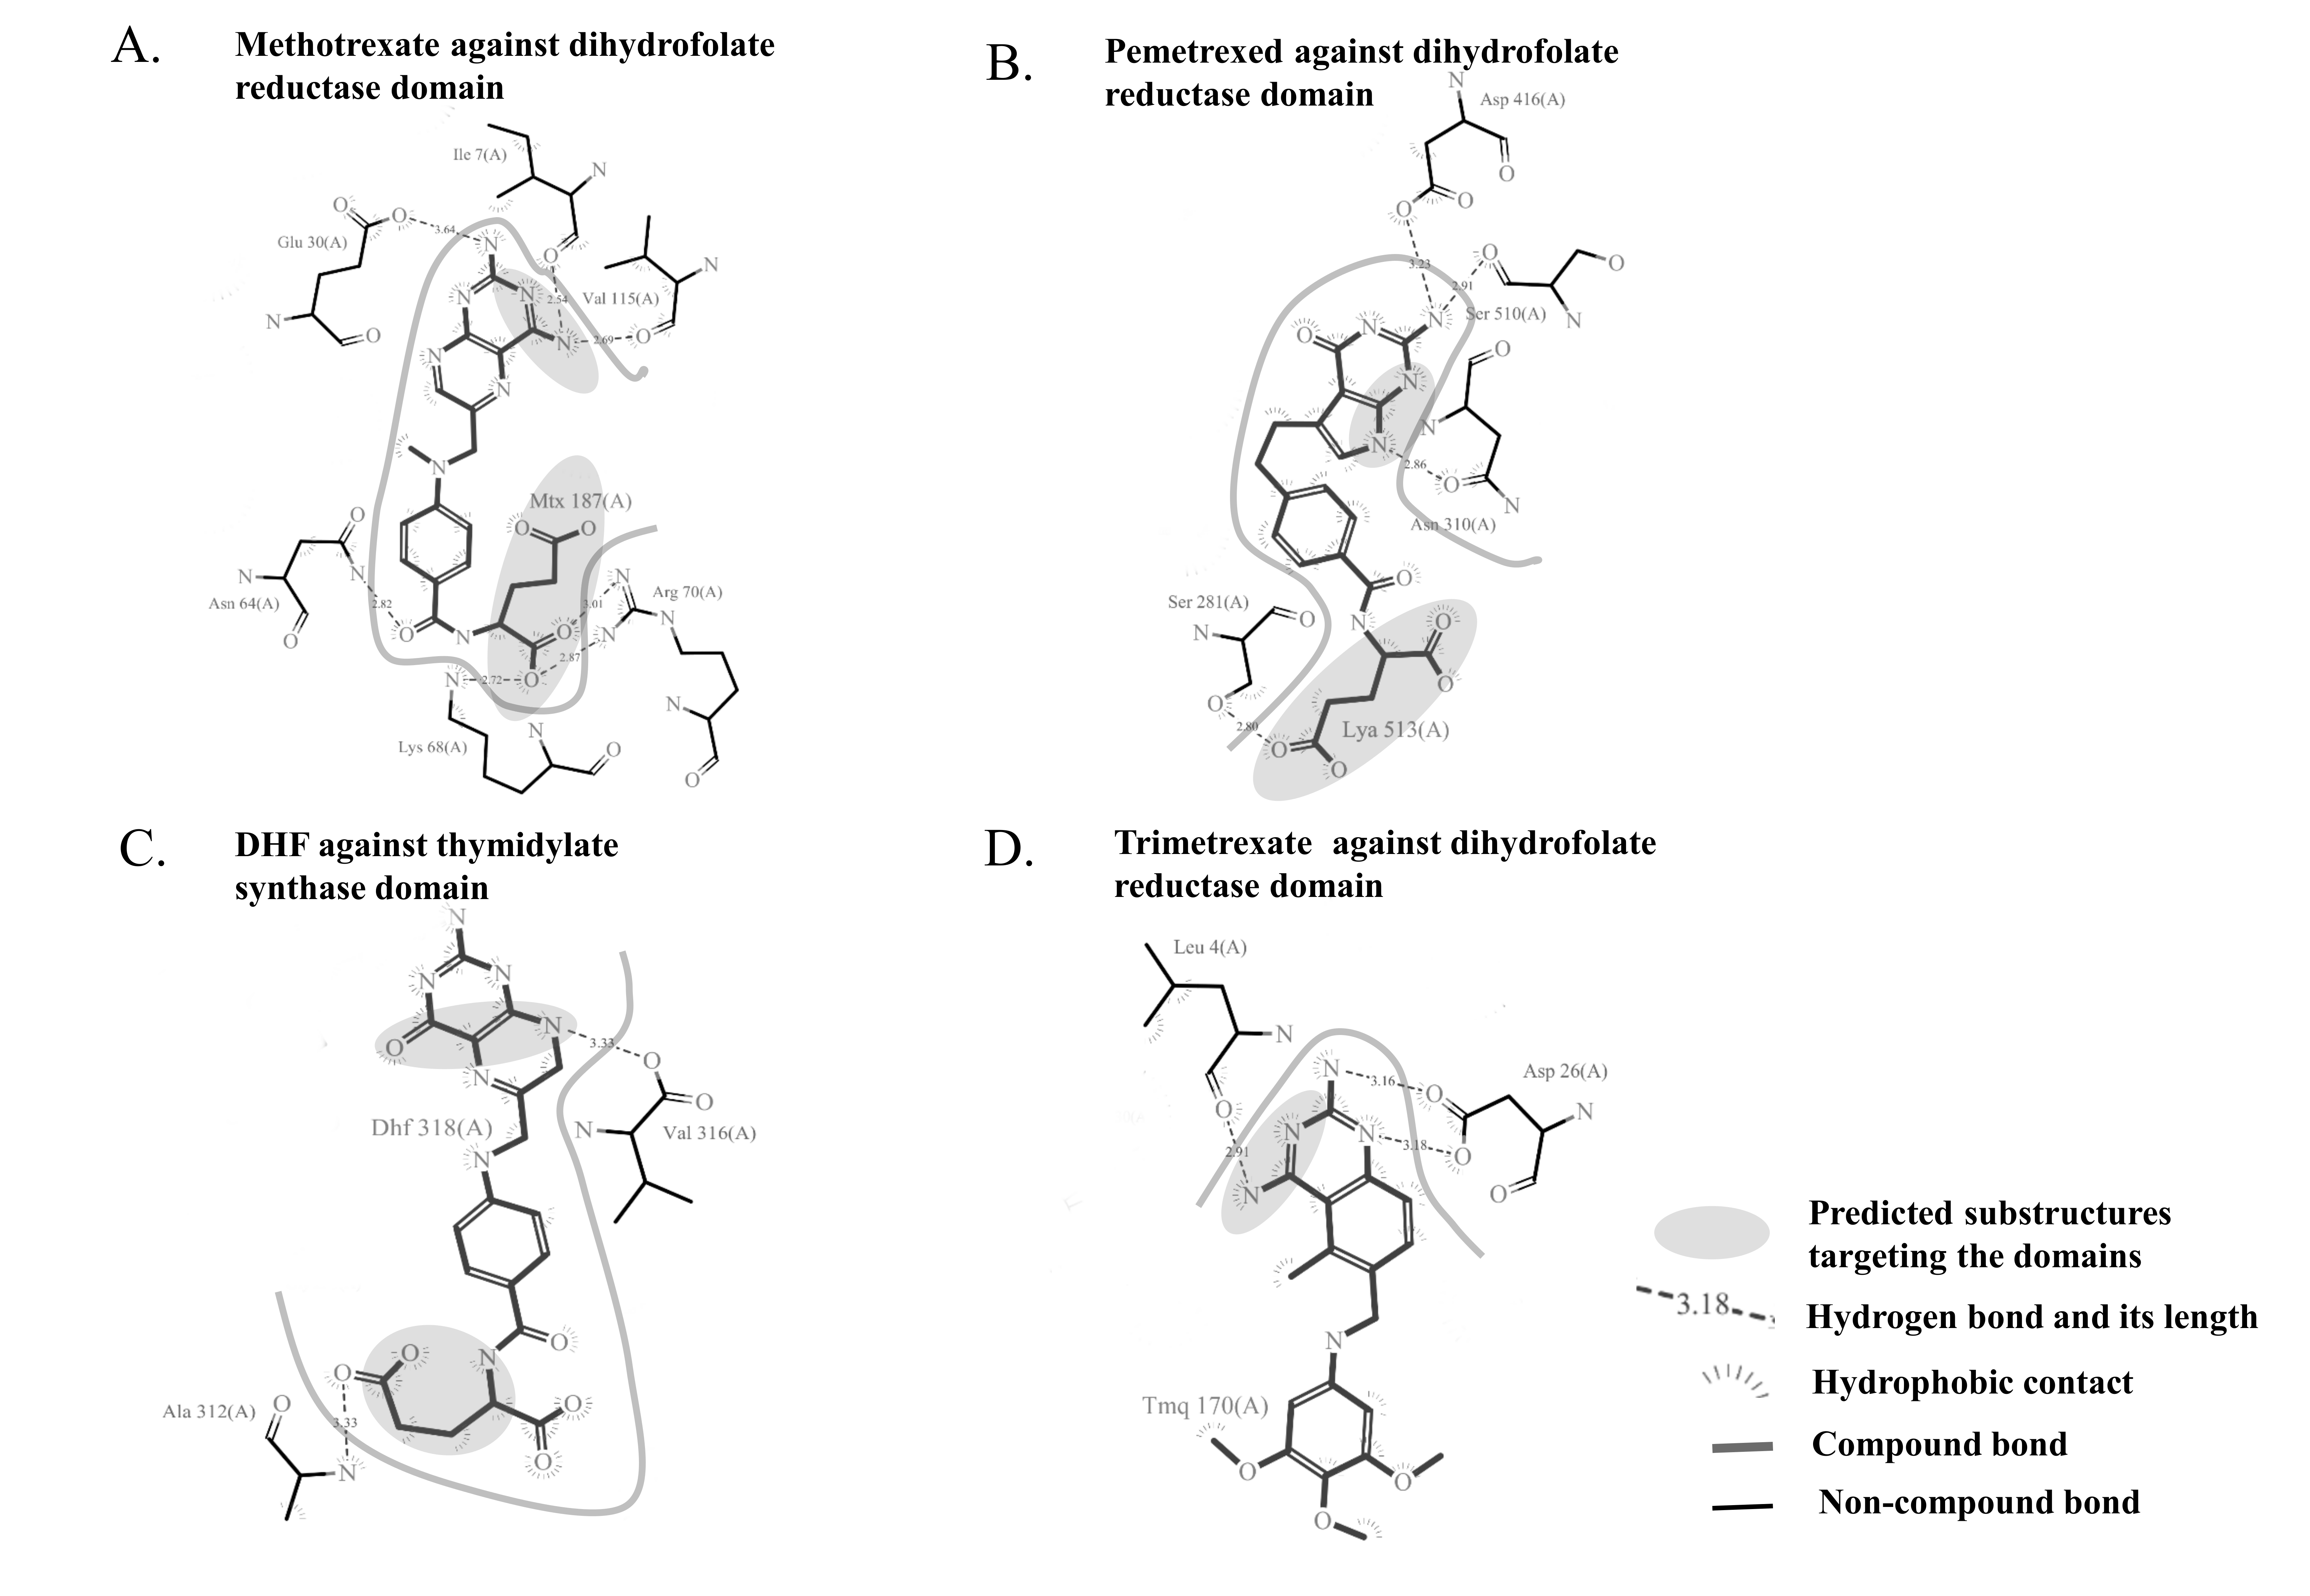
\includegraphics[width=0.8\textwidth]{ligplot_4_grey.png}}
\caption{Examples of the substructure-domain interactions validated from the Protein Data Bank database: (A) PDB entry 1u70, (B) PDB entry 3k2h, (C) PDB entry 1lcb, (D) PDB entry 1bzf. Dark grey: the drugs. Black: the amino acids. All the figures are generated by LigPlot (\citealp{wallace95}).
\label{fig:02}}
\end{figure*}

\begin{table*}
\processtable{Representative results of the predictions on drug-domain interactions.\label{Tab:03}}
{\begin{tabular}{ccccc}\toprule
Protein & Drug & Domain & k value & Prediction\\\midrule
DNA (cytosine-5)-methyltransferase 1 & S-Adenosylhomocysteine & C-5 cytosine-specific DNA methylase & 1 & TRUE \\
Alcohol dehydrogenase 1B & N-benzylformamide & Alcohol dehydrogenase GroES-like domain & 0.58 & TRUE\\
Androgen receptor & Flufenamic Acid & Ligand-binding domain of nuclear hormone receptor & 0.9 & TRUE\\
Ornithine carbamoyltransferase & N-(Phosphonoacetyl)-L-ornithine & Asp/Orn binding domain & 0.51 & TRUE\\
Progesterone receptor & Norethindrone & Ligand-binding domain of nuclear hormone receptor & 1 & TRUE\\
Rho-associated protein kinase 1 & hydroxyfasudil & Protein kinase domain & 0.94 & TRUE\\
Tissue-type plasminogen activator & benzamidine & Trypsin & 1 & TRUE\\\botrule
\end{tabular}
}{{\color{red}k value is the proportion of the number of the binding residues (amino acids) lying within the protein domain over the total number of the binding residues. When k value is larger than 0.5, the drug is considered to interact with the domain. TRUE means the prediction that the drug interacts with the domain by GIFT fits the real data well.}}
\end{table*}

\begin{table*}[ht]
\processtable{Results of the prediction interactions between drug chemical substructure combinations and protein domains.\label{Tab:04}}
{\begin{tabular}{ccccc}\toprule
Domain & Chemical Substructure & Chemical Substructure & Prediction (variance) & Proof from PDB\\\midrule
Eukaryotic-type carbonic anhydrase & N-S & Sc1cc(S)ccc1 & 1(0.21) & 1zgf\\
Dihydrofolate reductase & C($\sim$ N)(:C)(:N) & O-C-C-C-C-C-O & 0.32 (0.03) & 1u70 \\
Thymidylate synthase & O=C-C=C-N & O-C-C-C-C-N & 0.18 (0.01) & 1lcb\\
Dehydratase family & O($\sim$ C)($\sim$ P) & O=C-C=C-N & 0.18 (0.005) & 1n7h\\
Dihydrofolate reductase & C($\sim$Cl)(:C) & N-C-N-C:C & 0.17 (0.01) & 1j3j\\
Phosphoenolpyruvate carboxykinase & C($\sim$ N)(:C)(:N) & O=C-C-C-N & 0.17 (0.01) & 1khb \\
Cation transporting ATPase &	N-S	& Sc1cc(S)ccc1 & 0.16 (0.02) & 1zgf\\
5' nucleotidase family & C($\sim$C)(:N)(:N) & O-C-C-C-C-O & 0.15 (0.01) & 2xcw\\
Phosphorylase superfamily & N:C:N:C & O-C-C-O-[\#1] & 0.13 (0.005) & 1je1\\
Carbon-nitrogen hydrolase & C($\sim$ C)($\sim$ C)($\sim$ H)($\sim$ N) & O=C-C-C-C-C=O & 0.11 (0.006) & 3syt\\
Angiotensin-converting enzyme & O=C-C-N-C & O-C-C-C-C-C-N-C & 0.11 (0.002) & 1j37\\
Glutaminase & C($\sim$ C)($\sim$ C)($\sim$ H)($\sim$ N) & O=C-C-C-C-C=O & 0.11 (0.003) & 3vp0\\
Thymidylate synthase & C(-H)(-N)(=C) & O=C-N-C-[\# 1] & 0.08 (0.005) & 4fqs\\
GMP reductase domain & OC1CC(O)CCC1 & CC1C(C)CCCC1 & 0.08 (0.001) & 4fo4\\
Carboxylesterase & O-C:C-O-C & Cc1c(C)cccc1 & 0.08 (0.005) & 1eve\\\botrule
\end{tabular}}{ }
\end{table*}

\begin{figure*}
  \centering{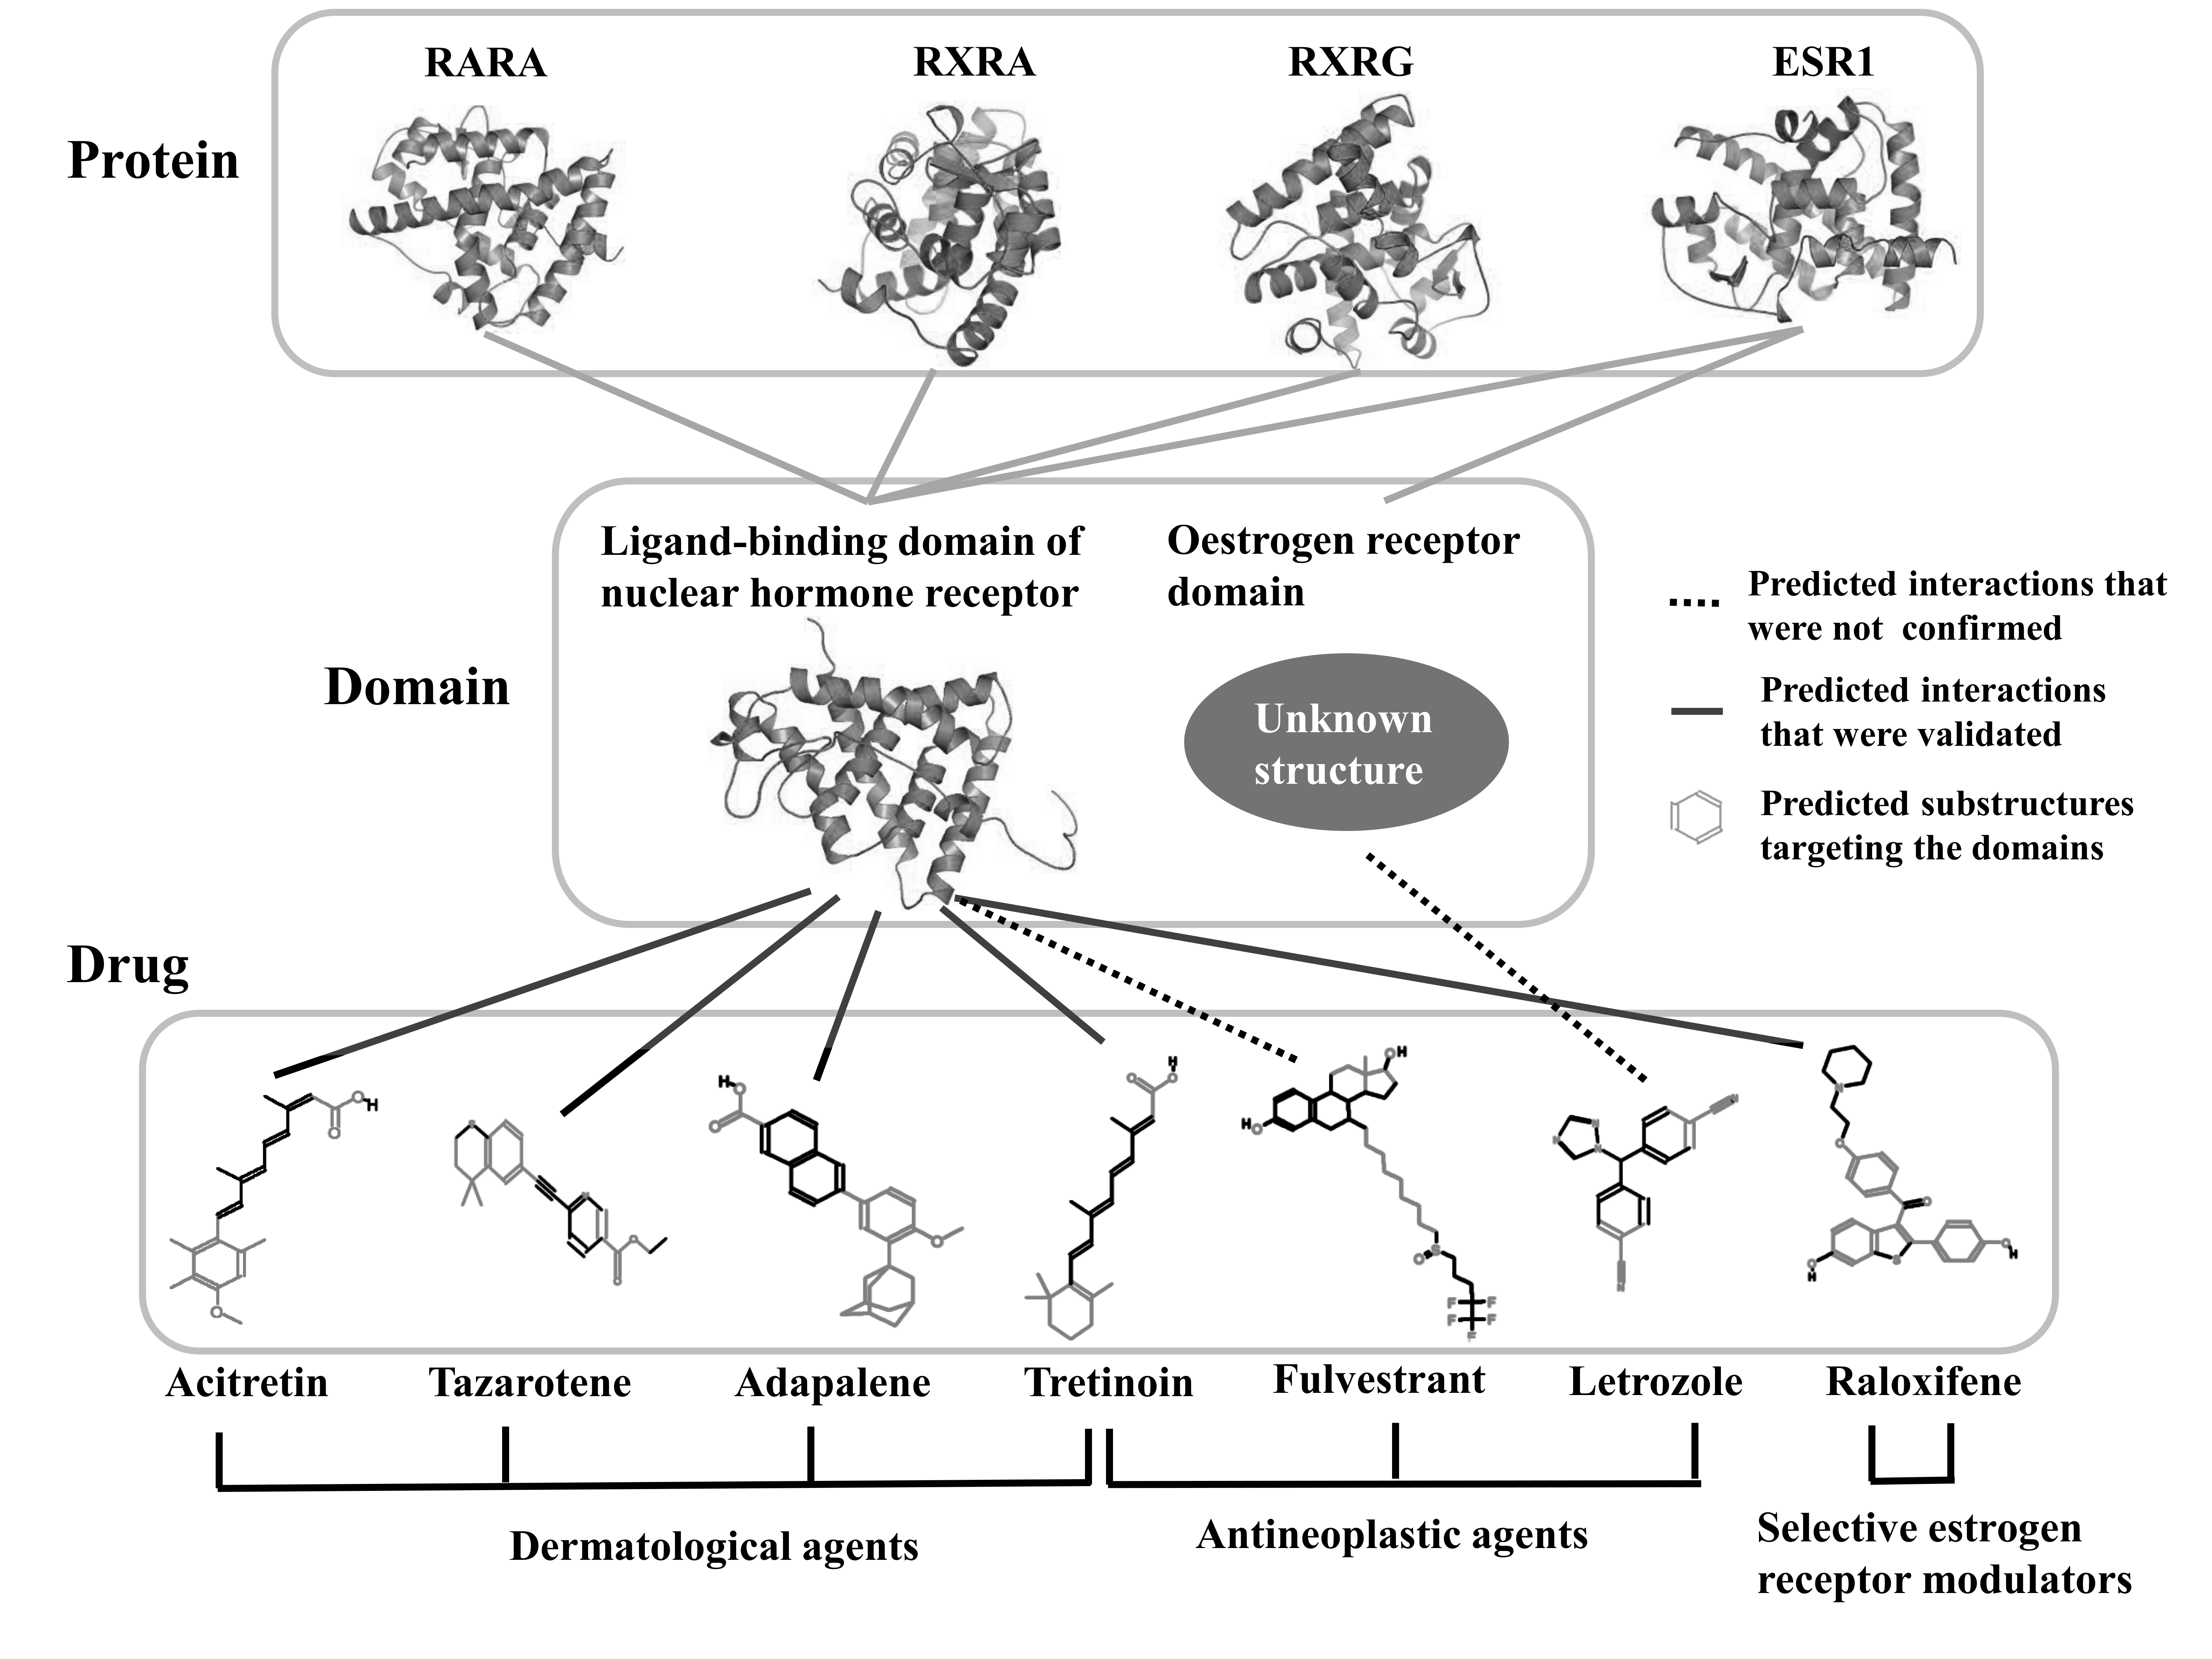
\includegraphics[width=0.8\textwidth]{MultiTarget_3_grey.png}}
  \caption{The example of connecting drug-protein interactions with the chemical substructure-domain interactions by GIFT.}
  \label{fig:03}
\end{figure*}

{\color{red}GIFT was then evaluated for its performance in predicting drug-domain interactions.} A total of 108 interactions between 53 proteins and 106 drugs were extracted from the crystallographic structures of known drug-protein interactions in the PDB database (\citealp{Kruger2012}). Domains coexisting in the same proteins were merged, so that only multidomain proteins were considered after data preprocessing. Finally 53 pairs of drug-protein interactions including 53 pairs of drug-domain interactions were left. {\color{red}Then the k value was used to describe the number of binding (amino acid) residues of a given drug were located in a given protein domain. Here k value was defined as the proportion of the number of the binding residuals lying within the protein domain over the total number of binding residuals, given a drug-target pair.} When k value was larger than 0.5, the drug was considered to interact with the domain (\citealp{Kruger14}).

The prediction of drug-domain interactions were followed Equation 2 in Methods, and each domain was treated as one protein. {\color{red}A drug and a protein domain were predicted to interact if the score given by GIFT was larger than zero.}

81\% of the drug-domain interactions could be predicted by GIFT. The representative results were shown in Table \ref{Tab:03}, and the complete results can be found in Supplementary Materials.

\subsection{Validation of Substructure-Domain Interactions}
A total of 726 substructure-domain interactions, whose scores, given by GIFT, were larger than their standard deviations, were extracted, including 255 interactions between substructure combinations and domains. Since some chemical substructures may function as one unit, more than 1800 combinations were recorded using the SMARTS format and added in our model (See Supplementary Material).

{\color{red}Interactions between combinations of chemical substructures and domains were validated by the known crystal complex containing the relevant drugs and proteins from the PDB database.} {\color{red}Eighteen} of the top 100 predicted interactions between combinations of chemical substructures and domains have the corresponding drug-target structures in the Protein Data Bank database, and 15 of {\color{red}the 18 ones} were successfully predicted (See Table \ref{Tab:04}).

Both methotrexate and pemetrexed are antitumor drugs (\citealp{DrugBank2008}), and can target against the dihydrofolate reductase and thymidylate synthase. One combination of the substructures interact with dihydrofolate reductase domain were predicted by GIFT, in good agreement with the real data (See Figure \ref{fig:02}A and \ref{fig:02}B). DHF, the methotrexate analog, can also interact with thymidylate synthase and showed the same results (See Figure \ref{fig:02}C). It was shown that methotrexate targeted two different domains with the same substructures. Trimetrexate is one agent against amoebiasis and other protozoal disease. Although it lacked one predicted substructure, when compared with methotrexate and pemetrexed, trimetrexate could still target against dihydrofolate reductase domain by the other predicted substructure(See Figure \ref{fig:02}D). Since it shares the same functional substructure with methotrexate and pemetrexed, trimetrexate may have similar biological activity. Indeed, it has been tested as an antitumor drugs (\citealp{DrugBank2008}).

\subsection{Interpretation of the Drug-Protein Interactions by GIFT}
We further explored the drug-protein interactions by GIFT, using four different proteins from Homo sapiens: RARA, RXRA, RXRG and ESR1. All have the ligand-binding domain of nuclear hormone receptor. ESR1 also contains the oestrogen receptor domain. Using GIFT, several chemical substructures were predicted to interact with the above domains. Drugs having these chemical substructures that can target at least one of the four proteins were shown in Figure \ref{fig:03}. In our data, tretinon, adapalene and acitretin targeted against RARA, RXRA and RXRG. Fulvestrant, raloxifene and letrozole interacted with ESR1. Tazarotene only targeted RARA. RARA shares the same protein domain as tretinon, adapalene and acitretin target RXRA and RXRG. Tazarotene might target the other two proteins. Based on the interpretation of GIFT, The four drugs also have the same chemical substructures predicted to target the ligand-binding domain of nuclear hormone receptor (labeled in red in Figure \ref{fig:03}) and they may, therefore, share the same therapeutic functions. Tretinoin has anticancer bioactivity. These results suggests that acitretin, adapalene, tazarotene and raloxifene may have similar anticancer activity similar to that of tretinoin.

Recent researches reported that adapalene could block cell proliferation and induce apoptosis on hepatoma cells (\citealp{Ocker04}). It was reported that tazarotene profoundly inhibits murine Basal cell carcinoma by inducing PI3K-AKT signaling (\citealp{So14}). Acitretin and several analogs exhibited antiproliferative activities against human breast MCF-7 epithelial cells (\citealp{Magoulas11}). Raloxifene, one of the selective estrogen-receptor modulators, was effective as a preventive choice in reducing the risk of breast cancer for postmenopausal woman (\citealp{Vogel10}).
\section{Discussion}
In this article, a statistic model, termed GIFT, was constructed to infer the interactions between drug chemical substructures and protein domains based on drug-protein interactions data. For the first time, a global optimization perspective has been introduced into this computation, meaning that all the substructure-domain contributions on drug-target interactions are simultaneously analyzed.

{\color{red}GIFT has several advantages compared with previous methods. First, it offers a more detailed description on the drug-protein interactions. Instead of adhering to the constraint which holds that "similar drugs target similar proteins", we attempt to reveal the possible mechanisms underlying drug-protein interactions. Second, more than 350,000 interactions were predicted by SCCA (\citealp{Yamanishi2011}), and around 5,000 interactions were predicted by L1-SVM (\citealp{Tabei2012}). However, these figures represent local estimates, in addition to the lack statistical significance evaluations, thus potentially overestimating substructure-domain interactions. GIFT, on the other hand, can reduce such overestimation by incorporating a global perspective that accommodates variance estimation. It should be noted that GIFT is limited in that it only focuses on two-dimensional chemical space, as presented by the 881 PubChem substructures. Therefore, in the future, three-dimensional structure information should be incorporated into the calculations (See Methods). As reflected by data already accumulated in the PDB database, more than 20,000 compound-protein interactions can be found, including more than 9,000 distinct compounds (\citealp{Gallina2013}; \citealp{deBeer2014}). Extraction of these binding information might result in more precise estimations of the substructure-domain interactions in the future.}

In summary, we propose a novel chemogenomic approach to infer substructure-domain interactions. It provides a chemogenomic view of the mechanisms of drug-protein interactions, and it can be used as a new method that contributes to target prediction, drug repositioning and drug combination studies.

\begin{methods}
\section{Methods}
\subsection{Data Sources of GIFT}
The information of drug-protein interactions, drug substructures, and protein domains is obtained from \citealp{Tabei2012}. A total of 1862 drugs are represented by 881-dimensional chemical substructure binary vectors from PubChem database, and 1554 proteins are represented by 876-dimensional protein domain binary vectors from the Pfam database (\citealp{Bateman04}). {\color{red}Here the substructure is defined as a specific kind of two-dimensional chemical fingerprint by CACTVS.} 4809 interactions exist between the drugs and the proteins. We deleted the drug chemical substructures or protein domains that never appeared in the drugs or proteins, and we merged those substructures or domains that appeared in the same drugs or proteins.

The drug-domain interactions were extracted from PDB database by the script from \citealp{Kruger2012}. We only chose proteins that had multiple domains for our data. Finally, 53 pairs of drug-protein interactions with the records of drug-domain interaction were used.
\subsection{The EM framework of GIFT}
Let $Y_1\ldots Y_T$ denote the T drugs, and $P_1\ldots P_S$ denote the S proteins.Let $Z_1\ldots Z_M$ denote the M drug chemical substructures and let $D_1\ldots D_N$ denote the N protein domains.Let $ZD^{(ij)}$ denote the set of the pairs of chemical substructures and domains from drug $Y_i$ and protein $P_j$ correspondingly. Let $ZD_{mn}$ denote the interaction result between the chemical substructure $D_m$ and the domain $D_n$.$ZD^{(ij)}_{mn} = 1$ if they interact and $ZD^{(ij)}_{mn}=0$ otherwise.Let $YP_{ij}$denotes the interaction result between the drug $Y_i$ and the protein $P_j$. $YP_{ij}=1$ if they interact and $YP_{ij}=0$ otherwise.

Inspired by the work \citealp{Minghua02}, we herein propose a statistical method to evaluate the possible interactions between drug chemical substructures and protein domains. For our calculations, it was assumed that 1) the interactions of the drug chemical substructures and the protein domains are independent, given a pair of a drug and a protein pair; 2) interactions between a given drug chemical substructure and protein domain would remain unchanged between different pairs of thedrugs and proteins containing them, as shown by
\begin{equation}
\theta_{mn} = Pr(D_{mn}^{(ij)}=1)
\end{equation}
in which $\theta_{mn} = Pr(D_{mn} = 1)$;
3) drug and the protein will interact if, and only if, one pair of chemical substructures and domains from them interact. Based on these assumptions, we can get
\begin{equation}
Pr(YP_{ij}=1|\theta)=1-\prod_{D_{mn}^{(ij)}}(1-\theta_{mn})
\end{equation}
We include two types of errors in the data of the drug protein interactions: \textit{fp} (false positive rate), in which the drug and the protein do not interact, but are recorded to be interacting, and \textit{fn} (false negative rate) , in which the drug and the protein interact, but are not recorded. Let $O_{ij}$ be the result of observed interaction between drug $Y_i$ and protein $P_j$:$O_{ij}=1$ if the interaction is observed and $O_{ij}=0$ otherwise.\\Then
\begin{eqnarray}
\textit{fp}=Pr(O_{ij}=1|YP_{ij}=0)\\
\textit{fn}=Pr(O_{ij}=0|YP_{ij}=1)
\end{eqnarray}
Both \textit{fn} and \textit{fp} are fixed in GIFT.
\begin{equation*}
\begin{aligned}
\textit{fn} &=Pr(O_{ij}=0|YP_{ij}=1)
=1- \frac{Pr(O_{ij}=1,YP_{ij}=1)}{Pr(YP_{ij}=1)}\\
&\geq 1- \frac{Pr(O_{ij}=1)}{Pr(YP_{ij}=1)}
\geq 1 - \frac{\text{number of observed interaction pairs}}{\text{number of real interaction pairs}}
\end{aligned}
\end{equation*}

It was estimated that on average the number of target proteins per drug was about 6.3 (\citealp{MEstres08}). The value of \textit{fn} then would be no less than 0.41. We estimate \textit{fp} in a similar way and it would be no more than 0.001.


And the probability for the observed interaction between drug $Y_{i}$ and the protein $P_{j}$ is
\begin{equation}
\begin{aligned}
Pr(O_{ij}&=1|\theta)=(1-\textit{fn})Pr(YP_{ij}=1|\theta)+\textit{fp}\cdot Pr(YP_{ij}=0|\theta)
%=(1-\textit{fn}-\textit{fp})Pr(YP_{ij}=1|\theta)+\textit{fp}
%&=Pr(O_{ij}=1|YP_{ij},\theta)Pr(YP_{ij}|\theta)\\
%&=Pr(O_{ij}=1|YP_{ij})Pr(YP_{ij}|\theta)\\
%&=Pr(O_{ij}=1|YP_{ij}=1)Pr(YP_{ij}=1|\theta)\\
%&\quad+Pr(O_{ij}=1|YP_{ij}=0)Pr(YP_{ij}=0|\theta)\\
%&=(1-\textit{fn})Pr(YP_{ij}=1|\theta)+\textit{fp}(1-Pr(YP_{ij}=1)|\theta))\\
%&=(1-\textit{fn}-\textit{fp})Pr(YP_{ij}=1|\theta)+\textit{fp}
\end{aligned}
\end{equation}
The log likelihood function is followed
\begin{equation}
\begin{aligned}
l(\theta)&=log(Pr(O|\theta))\\
%&=log(\prod_{all~i,j}{Pr(O_{ij}=1|\theta)^{O_{ij}}Pr(O_{ij}=0|\theta)^{1-O_{ij}}})
\end{aligned}
\end{equation}
It is a function of $\theta=\{\theta_{mn}\}$. $\theta$ is estimated by the maximum likelihood estimation approach. The Expectation-Maximization (EM) algorithm  (\citealp{dempster1977maximum}) is then used here.

The observed data are the interactions from DrugBank Database, $O = \{O_{ij}=o_{ij}\}$. The complete data include all the drug chemical substructures and protein domain interactions and the observed data. Let $A_m$ be the set of drugs containing the chemical substructure $Z_m$ and let $A_n$ be the set of proteins containing the domain $D_n$. Let $N_{mn}$ be the total number of pairs between $A_m$ and $A_n$. The EM algorithm as follows:\\
E Step:
\begin{equation}
  \begin{aligned}
    E(D_{mn}^{(ij)}|O,\theta^{(t-1)})
    &=\frac{\theta_{mn}^{(t-1)}(1-\textit{fn})^{O_{ij}}\textit{fn}^{1-O_{ij}}}{Pr(O_{ij}|\theta^{(t-1)})}
  \end{aligned}
\end{equation}
M Step:
\begin{equation}
\begin{aligned}
\theta_{mn}^{(t)}
&=\frac{1}{N_{mn}} \sum_{i,j: Zm\in Y_i, Dn\in P_j}E(D_{mn}^{(ij)}|O_{ij},\theta^{(t-1)})\\
%&=\frac{1}{N_{mn}}\sum_{i,j: Zm\in Y_i, Dn\in P_j}\frac{\theta_{mn}^{(t-1)}(1-\textit{fn})^{O_{ij}}\textit{fn}^{1-O_{ij}}}{Pr(O_{ij}|\theta^{(t-1)})}
\end{aligned}
\end{equation}
The variance of the parameters can be estimated by the observed Fisher information, which is followed:
\begin{equation}
var(\hat{\theta}) = \frac{1}{I(\hat{\theta})}, I(\theta) = -\frac{d^2 log(Pr(O|\theta))}{d{\theta}^2}
\end{equation}
Here $I(\hat{\theta})$ is the observed Fisher information.
In GIFT, the observed Fisher information is followed:
\begin{equation}
\begin{aligned}
I({\theta}_{mn})
%&= -\frac{{\partial}^2 log(Pr(O|\theta))}{\partial {\theta}_{mn}^2}\\
& = \sum_{i,j: Zm\in Y_i, Dn\in P_j}{\delta}_{mn}^{(i,j)^2}(\frac{O_{mn}^{(ij)}}{{\mu}_{mn}^{(ij)^2}}+\frac{1-O_{mn}^{(ij)}}{(1-{\mu}_{mn}^{(ij)})^2})
\end{aligned}
\end{equation}
In which,
\begin{equation}
%{\delta}_{mn}^{(ij)} = \frac{\partial Pr(O_{ij}^{(mn)}=1|\theta)}{\partial {\theta}_{mn}},
{\delta}_{mn}^{(ij)} = \frac{{\mu}_{mn}^{(ij)}}{\partial {\theta}_{mn}},
{\mu}_{mn}^{(ij)} = Pr(O_{mn}^{(ij)}=1|\theta)
\end{equation}
Since some drug chemical substructures may work as one unit, 1870 pairs of drug chemical substructures that frequently co-occur among the drugs are selected as the extra drug chemical substructures. All the details of GIFT can be found in our supplementary file.
\subsection{The Association Method}
The association method is A na\"{\i}ve way to estimate the interactions between chemical substructures and protein domain, which is the fraction of interacting drug-protein pairs among all of the drug-protein pairs containing the pair of chemical substructure $Z_m$ and protein domain $D_n$.
\begin{equation}
  \theta_{mn} = \frac{I_{mn}}{N_{mn}}
\end{equation}
in which $I_{mn}$ is the number of interacting pairs of drug-protein pairs containing the pair of chemical substructure $Z_m$ and protein domain $D_n$ and $N_{mn}$ is the number of total drug-protein pairs  containing the pair of chemical substructure $Z_m$ and protein domain $D_n$.

\end{methods}

\section*{Acknowledgement}
We thank Dr. Felix A Kruger at University of Cambridge for helpful discussion.
\paragraph{Funding\textcolon} This work is supported by NSFC (91229201 and 81225025).
\paragraph{Conflict of Interest\textcolon} none declared.

\begin{thebibliography}{}
\bibitem[Bateman {\it et~al}., 2004]{Bateman04} Bateman,A. {\it et~al}. (2004) The Pfam protein families database. \textit{Nucleic Acids. Res.}, \textbf{32}, D138-D141
\bibitem[Bemis {\it et~al}., 1996]{Bemis96} Bemis, GW. {\it et~al}. (1996) The properties of know drugs.1.Molecular frameworks. \textit{J.Med.Chem.} {\bf 39}, 2887-2893.
\bibitem[Bredel and Jacoy, 2004]{Bredel04}Bredel,M. and Jacoy,E. (2004) Chemogenomics: an emerging strategy for rapid target and drug discovery. \textit{ Nat. Rev. Genet.}, \textbf{5}, 262-275.
\bibitem[Berman {\it et~al}., 2000]{Berman00} Berman,HM. {\it et~al}. (2000) The protein data bank. \textit{Nucleic Acids. Res.}, \textbf{28}, 235-242.
\bibitem[Chothia, 1984]{Chothia84} Chothia,C. (1984) Principles that determine the structure of proteins. \textit{Annu.Rev.Biohem.}, {\bf 53}, 537-572.
\bibitem[Deng {\it et~al}., 2002]{Minghua02} Deng,M. \textit{et al}. (2002) Inferring Domain-Domain Interactions From Protein-Protein Interactions. \textit{Genome Res.}, {\bf 12}, 1540-1548.
\bibitem[de Beer {\it et~al}., 2014]{deBeer2014} de Beer,TA. {\it et~al}. (2014) PDBsum additions. \textit{Nucleic Acids. Res.}, \textbf{42}, D292--D296.
\bibitem[Dempster {\it et~al}., 1977]{dempster1977maximum} Dempster,A.P. \textit{et~al}. (1977) Maximum likelihood from incomplete data via the EM algorithm. \textit{J.R. Stat.Soc.Series.B.Stat.Methodol}, \textbf{39}, 1-38.
\bibitem[Duran-Frigola {\it et~al}., 2013]{duran13}Duran-Frigola,M. and Aloy,P. (2013) Analysis of chemical and biological features yields mechanistic insights into drug side effects. \textit{Chem. Biol.} \textbf{20}, 594-603.
\bibitem[Efron {\it et~al}., 1978]{efron78} Efron,B. {\it et~al}., (1978) Assessing the accuracy of the maximum likelihood estimator: Observed versus expected Fisher information. \textit{Biometrika}, \textbf{65}, 457-483.
\bibitem[Gallina {\it et~al}., 2013]{Gallina2013} Gallina,AM. {\it et~al}., (2013) PLI: a web-based tool for the comparison of protein-ligand interactions observed on PDB structures. \textit{Bioinformatics},\textbf{29}, 395-397.
\bibitem[Gaulton {\it et~al}., 2012]{gaulton2012} Gaulton,A. {\it et~al}., (2012) ChEMBL: a large-scale bioactivity database for drug discovery. \textit{Nucleic Acids. Res.}, \textbf{40}, D1100-D1107.
\bibitem[Geman {\it et~al}., 1984]{Geman84} Geman,S,. {\it et~al}., (1984) Stochastic Relaxation, Gibbs Distribution, and the Bayesian Restroration of Images. \textit{IEEE Trans. Pattern Anal. Mach. Intell.}
     \textbf{23}, 97-115.
\bibitem[James {\it et~al}., 1995]{James1995} James,C.A., Weininger,D., Delany,J. (1995) Daylight theory manual. Daylight chemical information systems, 3951.
\bibitem[Koehn and Carter, 2005]{Koehn2005} Koehn,F.E. and Carter G.T. (2005) The evolving role of natural products in drug discovery, \textit{Nat. Rev. Drug Discov.}, \textbf{4}, 206-220.
\bibitem[Kruger {\it et~al}., 2012]{Kruger2012} Kruger,F.A. {\it et~al}. (2012) Mapping small molecule binding data to structural domains. \textit{BMC Bioinformatics}, 13, Suppl 17, S11.
\bibitem[Kruger {\it et~al}., 2014]{Kruger14} Kruger,F.A. {\it et~al}. (2014) PPDMs - A resource for mapping small molecule bioactivities from ChEMBL to Pfam-A protein domains. \textit{Bioinformatics}.
\bibitem[Magoulas \textit{et~al}., 2011]{Magoulas11} Magoulas,G.E. \textit{et~al}. (2011) Syntheses, antiproliferative activity and theoretical characterization of acitretin-type retinoids with changes in the lipophilic part. \textit{Eur J Med Chem}, \textbf{46}, 721-737.
\bibitem[Mestres \textit{et~al}., 2008]{MEstres08}Mestres,J. \textit{et~al}. (2008) Data completeness--the Achilles heel of drug-target networks, \textit{Nat. Biotechnol}, \textbf{26}, 983-984.
\bibitem[Murray and Rees, 2009]{Murray09} Murray,C.W. and Rees, D.C. (2009) The rise of fragment-based drug discovery, \textit{Nat. Chem.}, \textbf{1}, 187-192.
\bibitem[Ocker \textit{et~al}., 2004]{Ocker04} Ocker,M. \textit{et~al}. (2004) Potentiated anticancer effects on hepatoma cells by the retinoid adapalene. \textit{Cancer Lett.}, \textbf{208}, 51-58.
\bibitem[So \textit{et~al}., 2014]{So14} So,P.L. \text{et~al}. (2014) PI3K-AKT Signaling Is a Downstream Effector of Retinoid Prevention of Murine Basal Cell Carcinogenesis, \textit{Cancer Prevention Research}, \textbf{7}, 407-417.
\bibitem[Sousa \textit{et~al}., 2013]{Sousa2013} Sousa,SF. \textit{et~al}. (2013) Protein-ligand docking in the new millennium--a restrospective of 10 years in the field. \textit{Curr. Med. Chem.}, \textbf{20}, 2296-2314.
\bibitem[Tabei \textit{et~al}., 2012]{Tabei2012} Tabei,Y. \textit{et~al}. (2012) Identification of chemogenomic features from drug--target interaction networks using interpretable classifiers. \textit{Bioinformatics}, \textbf{28}, i487-i494.
\bibitem[Takigawa {\it et~al}., 2011]{takigawa2011mining} Takigawa,I. \textit{et~al}., (2011) Mining significant substructure pairs for interpreting polypharmacology in drug-target network. \textit{PloS One}, \textbf{6}, e16999.
\bibitem[Vogel {\it et~al}., 2010]{Vogel10} Vogel,VG. \textit(et~al). (2010) Update of the national surgical adjuvant breast and bowel project study of tamoxifen and raloxifene (STAR) P-2 trial: preventing breast cancer. \textit{Cancer Prev Res}, \textbf{3}, 696-706.
\bibitem[Wang \textit{et~al}., 2009]{wang2009}Wang,Y. \textit{et~al}., (2009) PubChem: a public information system for analyzing bioactivities of small molecules. \textit{Nucleic Acids. Res.}, \textbf{37}, W623-633.
\bibitem[Wallace \textit{et~al}., 1995]{wallace95} Wallace,AC. \textit{et~al}., (1995) LIGPLOT: a program to generate schematic diagrams of protein-ligand interactions. \textit{Protein Eng.}, \textbf{8}, 127-134.
\bibitem[Wishart \textit{et~al}., 2008]{DrugBank2008} Wishart,DS. \textit{et~al}. (2008) DrugBank: a knowledgebase for drugs, drug actions and drug targets. \textit{Nucleic Acids. Res.}, \textbf{36}, D901-D906.
\bibitem[Yabuuchi {\it et~al}., 2011]{Hiroaki11} Yabuuchi,H. \textit{et~al}. (2011) Analysis of multiple compound-protein interactions reveals novel bioactive molecules. \textit{Mol.Syst.Biol.},\textbf{7}, 472.
\bibitem[Yamanishi \textit{et~al}., 2011]{Yamanishi2011} Yamanishi,Y. \textit{et~al}., (2011) Extracting sets of chemical substructures and protein domains governing drug-target interactions. \textit{J. Chem. Inf. Model.}, \textbf{51}, 1183-1184.
\bibitem[Yang {\it et~al}., 2013]{Yang2013} Yang, J., \textit{et~al}. (2013) Protein-ligand binding site recognition using complementary binding-specific substructure comparison and sequence profile alignment. \textit{Bioinformatics}, \textbf{29}, 2588-95.
\bibitem[Zhao and Li, 2010]{ZhaoS2010} Zhao,S. and Li,S. (2010) Network-based relating pharmacological and genomic spaces for drug target identification. \textit{Plos One}, \textbf{5},e11764.
\end{thebibliography}
\end{document}
